%!TeX root=../pridetop.tex
\chapter[Chapter \thechapter]{}
\begin{figure}[t!]
\centering
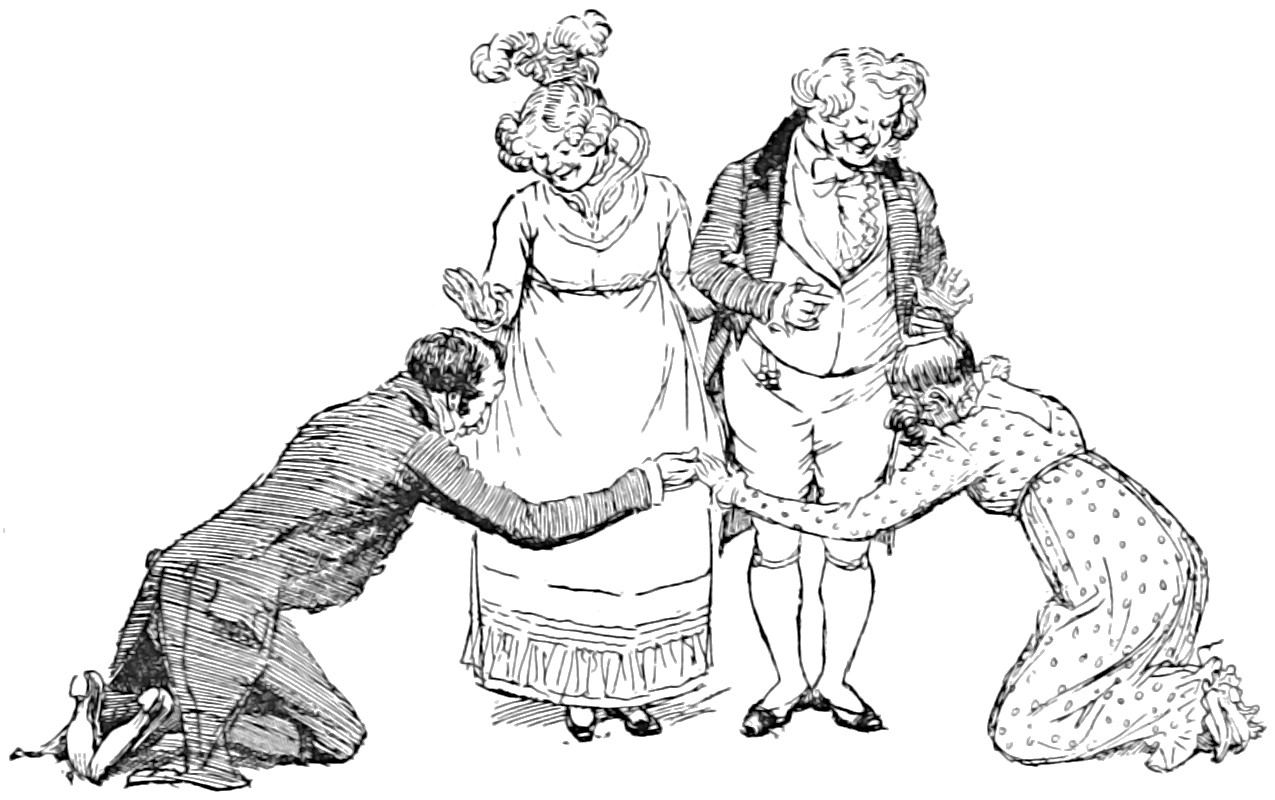
\includegraphics[width=\linewidth]{22top}
\captionlistentry{Headpiece to Chapter \thechapter}
\end{figure}


\lettrine[lines=6,image=true]{initials/chap22t}{he} Bennets were engaged to dine with the Lucases; and again, during the chief of the day, was Miss Lucas so kind as to listen to Mr Collins. Elizabeth took an opportunity of thanking her. 

\zz
<It keeps him in good humour,> said she, <and I am more obliged to you than I can express.>

\zz
Charlotte assured her friend of her satisfaction in being useful, and that it amply repaid her for the little sacrifice of her time. This was very amiable; but Charlotte's kindness extended farther than Elizabeth had any conception of:—its object was nothing less than to secure her from any return of Mr Collins's addresses, by engaging them towards herself. Such was Miss Lucas's scheme; and appearances were so favourable, that when they parted at night, she would have felt almost sure of success if he had not been to leave Hertfordshire so very soon. But here she did injustice to the fire and independence of his character; for it led him to escape out of Longbourn House the next morning with admirable slyness, and hasten to Lucas Lodge to throw himself at her feet. He was anxious to avoid the notice of his cousins, from a conviction that, if they saw him depart, they could not fail to conjecture his design, and he was not willing to have the attempt known till its success could be known likewise; for, though feeling almost secure, and with reason, for Charlotte had been tolerably encouraging, he was comparatively diffident since the adventure of Wednesday. His reception, however, was of the most flattering kind. Miss Lucas perceived him from an upper window as he walked towards the house, and instantly set out to meet him accidentally in the lane. But little had she dared to hope that so much love and eloquence awaited her there.

\begin{figure}[tbh!]
\centering
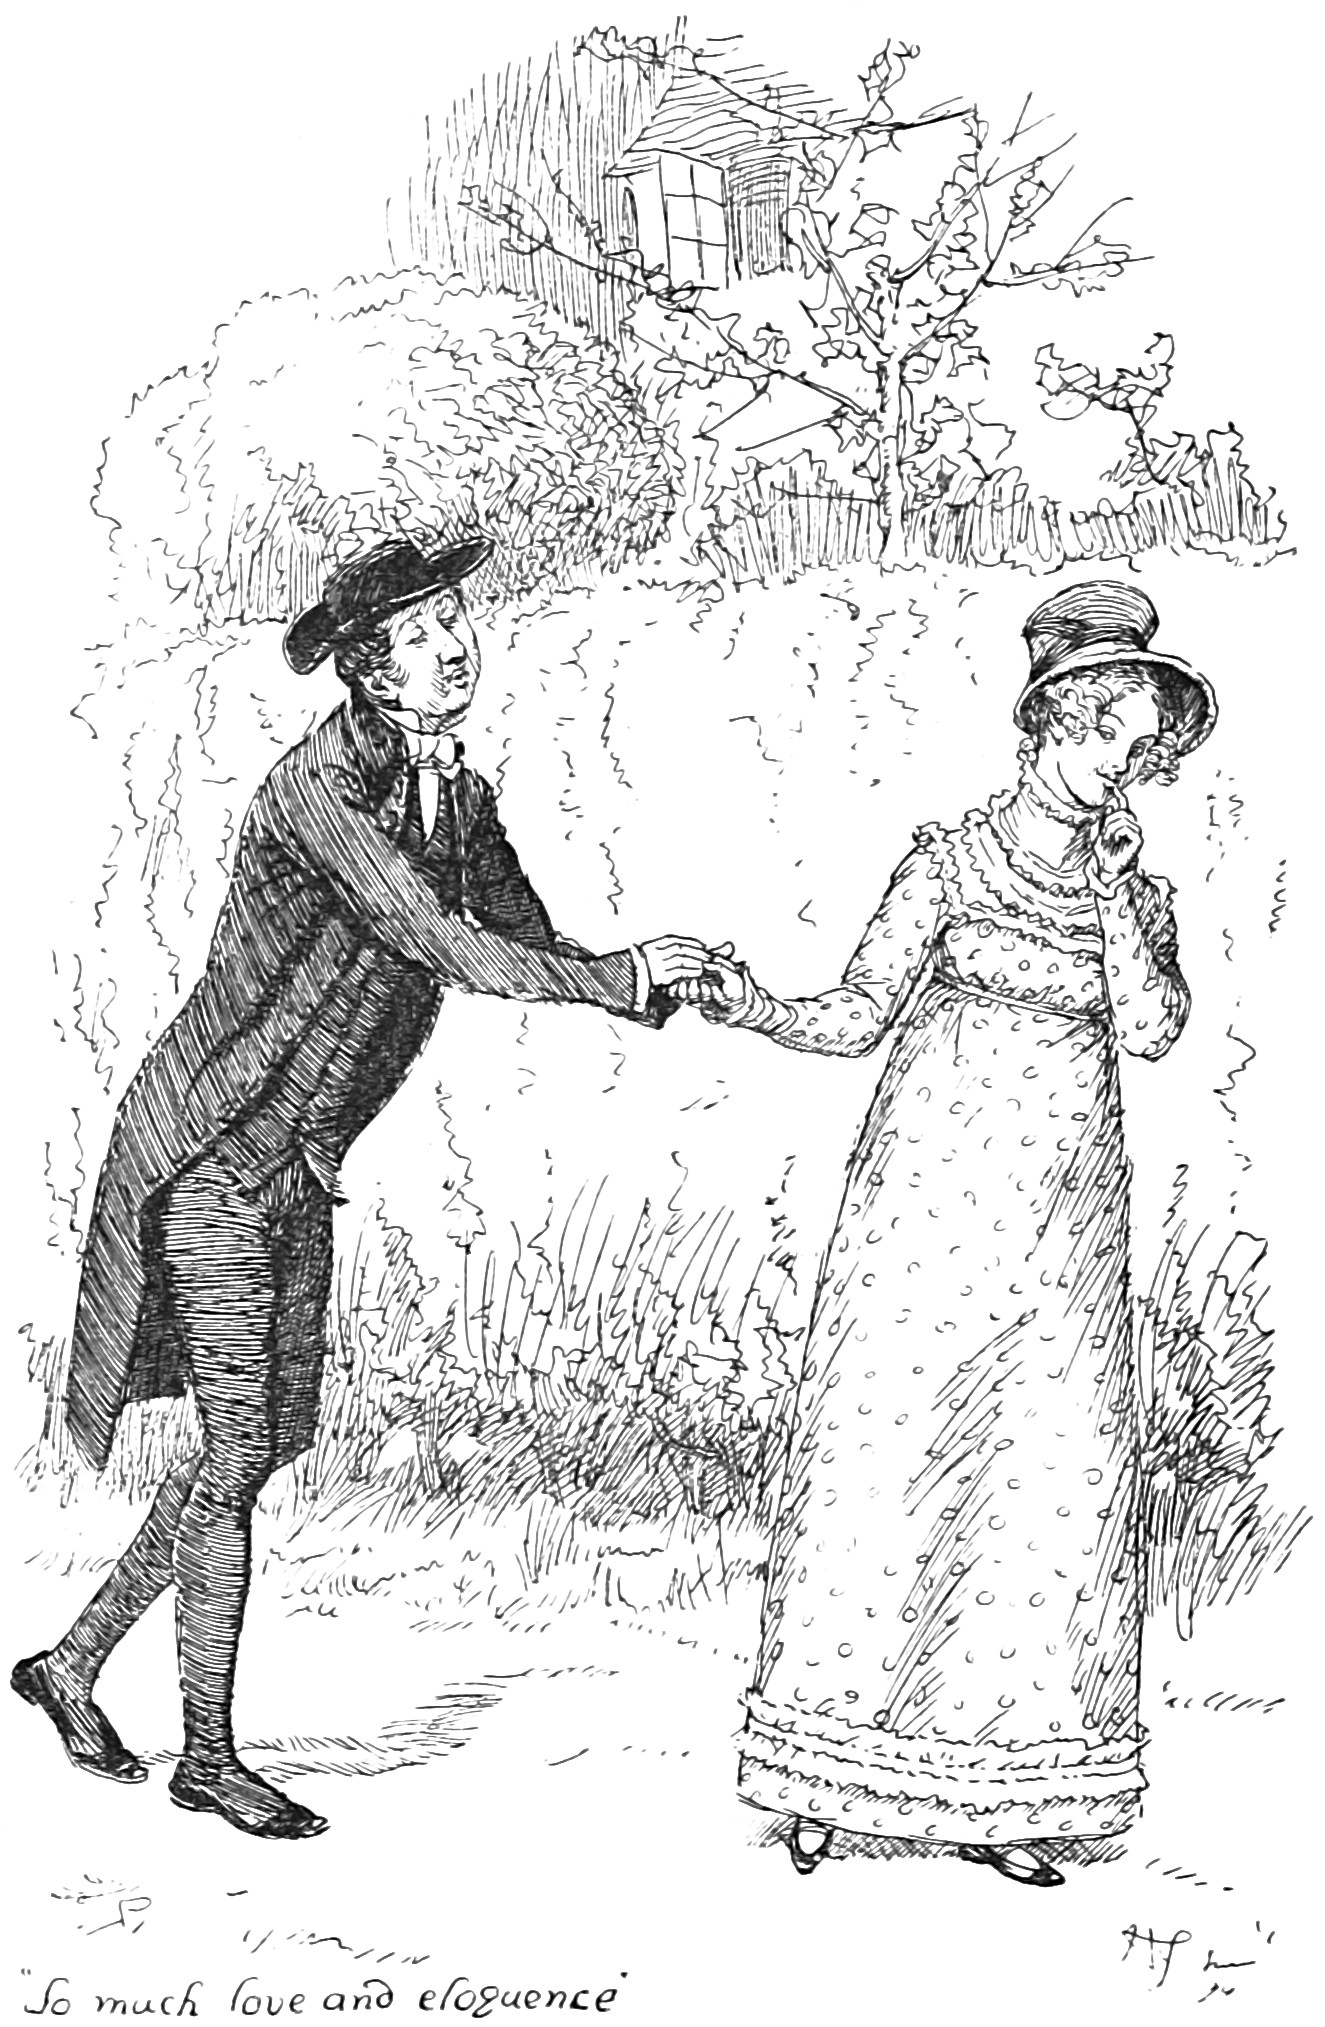
\includegraphics[width=.7\linewidth]{22love}
\captionlistentry{So much love and eloquence}
\end{figure}

In as short a time as Mr Collins's long speeches would allow, everything was settled between them to the satisfaction of both; and as they entered the house, he earnestly entreated her to name the day that was to make him the happiest of men; and though such a solicitation must be waived for the present, the lady felt no inclination to trifle with his happiness. The stupidity with which he was favoured by nature must guard his courtship from any charm that could make a woman wish for its continuance; and Miss Lucas, who accepted him solely from the pure and disinterested desire of an establishment, cared not how soon that establishment were gained.

Sir William and Lady Lucas were speedily applied to for their consent; and it was bestowed with a most joyful alacrity. Mr Collins's present circumstances made it a most eligible match for their daughter, to whom they could give little fortune; and his prospects of future wealth were exceedingly fair. Lady Lucas began directly to calculate, with more interest than the matter had ever excited before, how many years longer Mr Bennet was likely to live; and Sir William gave it as his decided opinion, that whenever Mr Collins should be in possession of the Longbourn estate, it would be highly expedient that both he and his wife should make their appearance at St James's. The whole family in short were properly overjoyed on the occasion. The younger girls formed hopes of \textit{coming out} a year or two sooner than they might otherwise have done; and the boys were relieved from their apprehension of Charlotte's dying an old maid. Charlotte herself was tolerably composed. She had gained her point, and had time to consider of it. Her reflections were in general satisfactory. Mr Collins, to be sure, was neither sensible nor agreeable: his society was irksome, and his attachment to her must be imaginary. But still he would be her husband. Without thinking highly either of men or of matrimony, marriage had always been her object: it was the only honourable provision for well-educated young women of small fortune, and, however uncertain of giving happiness, must be their pleasantest preservative from want. This preservative she had now obtained; and at the age of twenty-seven, without having ever been handsome, she felt all the good luck of it. The least agreeable circumstance in the business was the surprise it must occasion to Elizabeth Bennet, whose friendship she valued beyond that of any other person. Elizabeth would wonder, and probably would blame her; and though her resolution was not to be shaken, her feelings must be hurt by such a disapprobation. She resolved to give her the information herself; and therefore charged Mr Collins, when he returned to Longbourn to dinner, to drop no hint of what had passed before any of the family. A promise of secrecy was of course very dutifully given, but it could not be kept without difficulty; for the curiosity excited by his long absence burst forth in such very direct questions on his return, as required some ingenuity to evade, and he was at the same time exercising great self-denial, for he was longing to publish his prosperous love.

As he was to begin his journey too early on the morrow to see any of the family, the ceremony of leave-taking was performed when the ladies moved for the night; and Mrs Bennet, with great politeness and cordiality, said how happy they should be to see him at Longbourn again, whenever his other engagements might allow him to visit them.

<My dear madam,> he replied, <this invitation is particularly gratifying, because it is what I have been hoping to receive; and you may be very certain that I shall avail myself of it as soon as possible.>

They were all astonished; and Mr Bennet, who could by no means wish for so speedy a return, immediately said,—

<But is there not danger of Lady Catherine's disapprobation here, my good sir? You had better neglect your relations than run the risk of offending your patroness.>

<My dear sir,> replied Mr Collins, <I am particularly obliged to you for this friendly caution, and you may depend upon my not taking so material a step without her Ladyship's concurrence.>

<You cannot be too much on your guard. Risk anything rather than her displeasure; and if you find it likely to be raised by your coming to us again, which I should think exceedingly probable, stay quietly at home, and be satisfied that \textit{we} shall take no offence.>

<Believe me, my dear sir, my gratitude is warmly excited by such affectionate attention; and, depend upon it, you will speedily receive from me a letter of thanks for this as well as for every other mark of your regard during my stay in Hertfordshire. As for my fair cousins, though my absence may not be long enough to render it necessary, I shall now take the liberty of wishing them health and happiness, not excepting my cousin Elizabeth.>

With proper civilities, the ladies then withdrew; all of them equally surprised to find that he meditated a quick return. Mrs Bennet wished to understand by it that he thought of paying his addresses to one of her younger girls, and Mary might have been prevailed on to accept him. She rated his abilities much higher than any of the others: there was a solidity in his reflections which often struck her; and though by no means so clever as herself, she thought that, if encouraged to read and improve himself by such an example as hers, he might become a very agreeable companion. But on the following morning every hope of this kind was done away. Miss Lucas called soon after breakfast, and in a private conference with Elizabeth related the event of the day before.

The possibility of Mr Collins's fancying himself in love with her friend had once occurred to Elizabeth within the last day or two: but that Charlotte could encourage him seemed almost as far from possibility as that she could encourage him herself; and her astonishment was consequently so great as to overcome at first the bounds of decorum, and she could not help crying out,—

<Engaged to Mr Collins! my dear Charlotte, impossible!>

The steady countenance which Miss Lucas had commanded in telling her story gave way to a momentary confusion here on receiving so direct a reproach; though, as it was no more than she expected, she soon regained her composure, and calmly replied,—

<Why should you be surprised, my dear Eliza? Do you think it incredible that Mr Collins should be able to procure any woman's good opinion, because he was not so happy as to succeed with you?>

But Elizabeth had now recollected herself; and, making a strong effort for it, was able to assure her, with tolerable firmness, that the prospect of their relationship was highly grateful to her, and that she wished her all imaginable happiness.

<I see what you are feeling,> replied Charlotte; <you must be surprised, very much surprised, so lately as Mr Collins was wishing to marry you. But when you have had time to think it all over, I hope you will be satisfied with what I have done. I am not romantic, you know. I never was. I ask only a comfortable home; and, considering Mr Collins's character, connections, and situation in life, I am convinced that my chance of happiness with him is as fair as most people can boast on entering the marriage state.>

Elizabeth quietly answered <undoubtedly;> and, after an awkward pause, they returned to the rest of the family. Charlotte did not stay much longer; and Elizabeth was then left to reflect on what she had heard. It was a long time before she became at all reconciled to the idea of so unsuitable a match. The strangeness of Mr Collins's making two offers of marriage within three days was nothing in comparison of his being now accepted. She had always felt that Charlotte's opinion of matrimony was not exactly like her own; but she could not have supposed it possible that, when called into action, she would have sacrificed every better feeling to worldly advantage. Charlotte, the wife of Mr Collins, was a most humiliating picture! And to the pang of a friend disgracing herself, and sunk in her esteem, was added the distressing conviction that it was impossible for that friend to be tolerably happy in the lot she had chosen.